%%%%%%%%%%%%%%%%%%%%%%%%%%%%%%%%%%%%%%%%%%%%%%%%%%%%%%%%%%%%
%% Chapter 1 - Introduction (indicative length: 6-9 pages)
%% Purpose: introduce the practical and scientific problem,
%% motivate the proposed learning-based adaptive architecture,
%% and state exactly what the thesis contributes.
%% Main output: research problem, research questions,
%% objectives, contributions, scope, and chapter roadmap.
%%%%%%%%%%%%%%%%%%%%%%%%%%%%%%%%%%%%%%%%%%%%%%%%%%%%%%%%%%%%
\chapter{Introduction}
\label{chap:introduction}

\section{The Role of Mechanised Verge Maintenance}
\label{sec:intro:verge}

Road verges are cut because they are infrastructure. Vegetation left to grow
closes sight lines at junctions and bends, obscures signs and barriers, blocks
the drainage channels that keep water off the carriageway, and encroaches on the
running surface itself. A national road network carries tens of thousands of
kilometres of verge, and each kilometre is cut several times in a growing
season, so the work is continuous, repetitive and performed almost entirely by
machine.

It is also performed from a moving vehicle. Stopping to cut each section would
require closing the lane, so a carrier drives the road at a few kilometres per
hour while a boom-mounted mowing head works the verge alongside it. The head
must hold a cut height of a few centimetres over ground that rises and falls
continuously, follow a grass line that curves with the road, and do so without
striking the surface hard enough to damage the tool or lift the machine.

The demands on the manipulator follow from that. The machine studied here,
shown in Figure~\ref{fig:intro:fme500}, carries a heavy rotating tool at the end
of a long boom, works in intermittent contact with the ground,
and must place that tool accurately while its own base is in motion. Hydraulic
actuation is the standard answer at this scale: it supplies the force density
and the tolerance to shock loading that electric drives do not, and it does so
with components rugged enough for continuous outdoor operation. Precision,
however, is not what hydraulics are good at, and that tension is the subject of
this thesis.

\section{Advances in Learning-Based Control for Hydraulic Manipulators}
\label{sec:intro:advances}

Two developments have changed what is achievable on machines of this kind.

The first is that policy optimisation in simulation has become practical for
contact-rich manipulation. GPU-parallel physics engines run thousands of
environments simultaneously, which makes reinforcement learning feasible on
tasks that would take years of real-machine experience, and randomising the
simulator across a family of plants produces policies that transfer without
being tuned to one machine. The second is that the actuator itself can be
learned. Rather than deriving valve and cylinder behaviour from first principles
and fitting its parameters, a network trained on recorded motion can represent
the command-to-motion relationship directly, including the nonlinearities that
analytical models approximate away. Chapter~\ref{chap:fundamentals} sets out
both lines and the work they rest on.

Combining the two is attractive and not straightforward. A learned actuator
model must be cheap enough to evaluate inside the training loop, which rules out
the high-fidelity models used for offline analysis, and it must remain valid
across the family of machines the policy will meet. This has motivated a line of
work in which a compact code describing the current plant is inferred from
recent interaction history and supplied to the controller, so that a single
policy can serve a family rather than a single
machine. Such methods report substantial gains in legged locomotion and in
manipulation, and they are the direct antecedent of the architecture examined
here.

\begin{figure}[H]
  \centering
  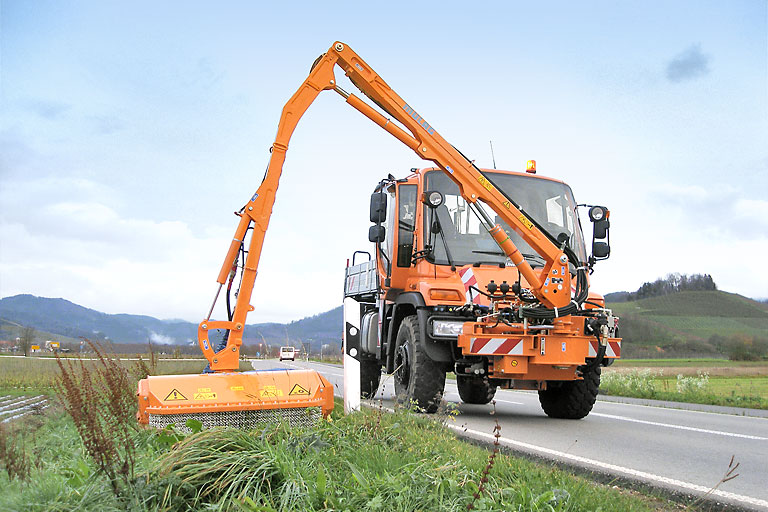
\includegraphics[width=.82\textwidth]{images/ch1/fme500_operation}
  \caption{MULAG FME~500 front mower on a Unimog during roadside verge
  maintenance. Image source: MULAG Fahrzeugwerk, FME~500 product
  documentation.}
  \label{fig:intro:fme500}
\end{figure}

\section{Challenges of Precise Tracking with Hydraulic Mowing Arms}
\label{sec:intro:challenges}

A valve command does not produce a proportional cylinder motion. The
relationship is nonlinear, depends on load and supply pressure, and is subject
to dead time between the command and any measurable response. It also differs
between machines: seal condition, fluid temperature, hose compliance and the
attachment fitted all change it, so two machines of the same model respond
differently and one machine responds differently across a season. A controller
that inverts only the geometry therefore leaves the largest source of tracking
error unaddressed.

That difficulty admits two responses, and they are routinely conflated. The
first is robustness: train across a randomised family so that a single fixed
model is adequate everywhere. It costs nothing at run time and gives up the
difference between the family and the individual. The second is adaptation:
infer which member of the family is present from the interaction history and
condition the model or the policy on that estimate. It promises to recover
that
difference, at the cost of an estimator that must work from observable signals
alone, since a deployed machine has no access to its own plant parameters.

Whether adaptation repays that cost depends on three things. Plant identity must
be present in the signals produced under the available excitation. The robust
controller must leave a control-relevant deficit to recover. The correction
path must retain enough authority to change the realised command. This thesis
measures these conditions on a hydraulic mowing arm and then evaluates whether
an online estimate of the operating condition improves closed-loop tracking.

\section{Contribution of This Thesis}
\label{sec:intro:contributions}

The difficulty described in Section~\ref{sec:intro:challenges} is a modelling
problem before it is a control problem. A hydraulic actuator can be simulated
accurately, but the models that do so are too slow to sit inside a
reinforcement-learning loop requiring millions of environment steps, while the
usual alternative of commanding joint positions directly removes the load and
pressure dependence that makes the machine difficult to control. What is needed
is a representation cheap enough to train against and faithful enough that the
resulting policy controls something close to the real actuator.

Learned actuator models and payload-conditioned adaptation are both established
techniques. What remains unclear is how such models should be identified so that
they retain the command dependence a controller needs, whether they transfer
between simulators without retraining, and what a controller must know about its
load once the models are used in control. Representation and transfer are
established first because the adaptation acts through an identified actuator
model rather than replacing one. Online adaptation is evaluated last so that any remaining
gain can be interpreted against the transferred model and the robustness of the
fixed controller. The order follows the dependencies among the claims. The
research statement is as follows:

\paragraph{Comparison notation.}
Three policy--actuator stacks are compared, each carrying a short label used
throughout. \emph{R} (\ppoROMfull) uses the command-conditioned reduced-order
model. \emph{IF} (\ppoIDFDfull) uses the frozen inverse and forward pair.
\emph{AF} (\ppoAAMFDfull) drops the inverse model and commands the valve
directly, which is where command authority remains. The labels name complete stacks rather than actuator models
alone, and Section~\ref{sec:ctrl:ppo-aamfd} gives their construction. One point
is worth fixing here because the name invites the opposite reading: the offline
AAM of Chapter~\ref{chap:models} is a diagnostic estimator and is not loaded in
the AF command path.

\researchstatement{To determine how hydraulic actuator dynamics learned from
high-fidelity simulation can be reduced, transferred into a computationally
efficient robotic simulation and used for reinforcement-learning control, and
under what conditions online adaptation improves on the robustness those learned
models already provide.}

The statement decomposes into six research questions, which are answered in the
order given. The first three concern how the actuator is represented, the fourth
concerns control through that representation, and the last two concern what
remains for adaptation once the first four are settled. The six questions are:

\begin{enumerate}
  \item How can data from a high-fidelity Simscape model be used to learn
    computationally tractable representations of hydraulic actuation while
    preserving the command dependence a controller requires?
  \item To what extent do actuator models identified from Simscape transfer to
    an IsaacLab manipulator without deployment-specific retraining?
  \item Can a structurally constrained reduced-order hydraulic model supply
    dynamics that are accurate and stable enough for GPU-parallel policy
    training?
  \item Can a policy trained from a privileged classical teacher become the sole
    deployed controller while acting through learned actuator dynamics?
  \item How does the choice of actuator representation affect tracking, command
    behaviour, latency and robustness under plant variation?
  \item Where plant variation survives robust training, can a controller
    estimate its own payload online and condition on it, and in which regime
    does that conditioning improve closed-loop tracking rather than cost it?
\end{enumerate}

RQ6 concerns one deployed mechanism. The policy receives a payload estimate
computed at runtime from the task observation it already carries, and only the
context columns of an otherwise frozen policy are trained, so zeroing the
estimate recovers the frozen controller exactly
(Section~\ref{sec:ctrl:af-residual}). What the policy is given is a single
physical quantity rather than an unconstrained code, and it is tested as such.
The AAM of Section~\ref{sec:models:aam} is not part of this path. It is an
offline diagnostic used to judge whether the inverse model can be trusted, and
the frozen stacks are robust controllers rather than adaptive ones.

The first question is answered in Chapters~\ref{chap:data}
and~\ref{chap:models}, the second and third in Chapter~\ref{chap:models}, the
fourth in Chapter~\ref{chap:control}, and the last two in
Chapter~\ref{chap:evaluation}.

RQ6 is the question named in the title and is deliberately placed last, since it
is only worth asking once the preceding questions have established that the
learned models transfer, that a policy can control through them, and how much
plant variation the closed loop already absorbs unaided. Its answer separates
two levels. Online plant context is usable at the model level, and whether that
benefit reaches the closed loop depends on the interface the correction acts
through: plant variation must remain control-relevant after robust training, be
observable from the available history, and reach a correction path with
sufficient authority. Any apparent gain must also be separated from the effect
of conditioning on a plausible load rather than the correct one. The work rests on the following contributions:

\textbf{Transferable Hydraulic Actuator Learning:} A pipeline that identifies
hydraulic actuation from high-fidelity Simscape data and transfers it into
IsaacLab through two representations, a modular inverse and forward chain and a
structurally constrained reduced-order model. The inverse and forward pair transfers
frozen, without deployment-specific retraining. The reduced-order model instead
receives a small bounded calibration against the deployment plant, so it serves
as a reference condition rather than an independent competitor
(Chapter~\ref{chap:models}).

\textbf{Control-Relevant Identification and Validation:} A demonstration that
predictive accuracy can conceal the loss of exactly the property a controller
needs, together with the procedure that detects it. A forward model reached a
near-perfect supervised score while learning to ignore the valve command. The
validation loss did not show this; ablating the command did. Excitation design
paired with input ablation is established here as a required test before a
learned actuator model is admitted to control
(Chapters~\ref{chap:data} and~\ref{chap:models}).

\textbf{Reduced-Order Actuator Model:} A command-conditioned recurrent actuator
surrogate whose transition is written as an explicit hydraulic chain, so the
predicted step stays differentiable in named quantities and bounded in form,
with learned heads covering valve realisation and unmodelled loading. It is
accurate enough to serve as the deployment plant, stable in recursive rollout,
and cheap enough to evaluate inside GPU-parallel policy training. It is not an
identified plant: the fitted physical constants settle on their clamps and the
realised motion comes from the learned heads, which is measured and reported
rather than assumed (Section~\ref{sec:models:rom}).

\textbf{Policy-Only Control Through Learned Hydraulics:} A damped least-squares
controller supplies privileged demonstrations during training and is then
removed, leaving the distilled policy as the entire deployed controller, acting
through learned actuator dynamics. Both representations support closed-loop
terrain following in that configuration
(Chapters~\ref{chap:control} and~\ref{chap:evaluation}). One training run
exists per representation, so this compares two realised controllers and does
not estimate what retraining either would produce.

\textbf{A Decision Procedure for Online Adaptation:} A matched protocol that
asks, in order, whether plant identity is present in the identification data,
what a privileged plant encoding does in the closed loop, and only then fits a
deployable estimator of it. Either of the first two measurements can show that a
correction would have nothing to act on
(Chapters~\ref{chap:models} and~\ref{chap:evaluation}).

\textbf{Where Online Adaptation Is Effective:} An online payload-conditioned
controller measured on one machine under one protocol, with the regime in which
it helps identified rather than assumed. It improves cut height, lateral
tracking and ground contact together where a heavy payload costs the frozen
controller ground contact, and costs lateral accuracy where the frozen
controller is not failing. Permuting the payload across environments separates
what correct identification contributes from what conditioning on any plausible
load contributes (Chapter~\ref{chap:evaluation}).

Chapter~\ref{chap:conclusion} restates these six with the measurements attached.
They are stated here as claims and there as results, so the evidence is given
once.

The causal plant estimator, the bounded adaptation path and the eight-gate
evaluation harness are described where they are used, as technical enablers
rather than separate claims.

Figure~\ref{fig:intro:research-cycle} condenses the logic that connects these
contributions. The sequence is a cycle rather than a one-way pipeline: evidence
from robustness, identifiability and adaptation feeds back into the next
actuator representation and the transfer assumptions made for it.

\begin{figure}[H]
  \centering
  \resizebox{.80\textwidth}{!}{\begin{tikzpicture}[
  x=1cm,
  y=1cm,
  cyclearc/.style={-{Triangle[length=3.2mm,width=4.0mm]},
    line width=5.2pt,line cap=round},
  cyclelabel/.style={align=center,text width=2.90cm,
    font=\small\bfseries,text=black!82}
]
  % A pale uninterrupted track makes the circular structure explicit.
  \draw[draw=black!10,line width=8.2pt]
    (90:4.45) arc[start angle=90,end angle=-270,radius=4.45];

  % Six clockwise arcs form one closed cycle. Small gaps keep each arrowhead
  % distinct while the background track preserves continuity.
  \draw[cyclearc,draw=cbblue!88!black]
    (86:4.45) arc[start angle=86,end angle=34,radius=4.45];
  \draw[cyclearc,draw=cbpink!88!black]
    (26:4.45) arc[start angle=26,end angle=-26,radius=4.45];
  \draw[cyclearc,draw=cborange!95!black]
    (-34:4.45) arc[start angle=-34,end angle=-86,radius=4.45];
  \draw[cyclearc,draw=cbgreen!82!black]
    (-94:4.45) arc[start angle=-94,end angle=-146,radius=4.45];
  \draw[cyclearc,draw=cbblue!62!black]
    (-154:4.45) arc[start angle=-154,end angle=-206,radius=4.45];
  \draw[cyclearc,draw=cbpink!72!black]
    (-214:4.45) arc[start angle=-214,end angle=-266,radius=4.45];

  \node[cyclelabel] at (90:2.95)
    {\textcolor{cbblue!88!black}{\normalsize 1.}\\[-1pt]
     Actuator\\representation};
  \node[cyclelabel] at (30:2.95)
    {\textcolor{cbpink!88!black}{\normalsize 2.}\\[-1pt]Transfer};
  \node[cyclelabel] at (-30:2.95)
    {\textcolor{cborange!95!black}{\normalsize 3.}\\[-1pt]Control};
  \node[cyclelabel] at (-90:2.95)
    {\textcolor{cbgreen!82!black}{\normalsize 4.}\\[-1pt]Robustness};
  \node[cyclelabel] at (-150:2.95)
    {\textcolor{cbblue!62!black}{\normalsize 5.}\\[-1pt]Identifiability};
  \node[cyclelabel] at (150:2.95)
    {\textcolor{cbpink!72!black}{\normalsize 6.}\\[-1pt]Adaptation};

  \node[circle,draw=cbblue!80!black,line width=1pt,fill=cbblue!7,
    minimum size=2.65cm,align=center,font=\normalsize\bfseries,
    text=cbblue!75!black] at (0,0)
    {Thesis research\\cycle};
\end{tikzpicture}
}
  \caption{Research cycle connecting actuator representation, transfer,
  closed-loop control, robustness, identifiability, and adaptation. Evidence
  from the final stages informs the next actuator representation and its transfer
  assumptions.}
  \label{fig:intro:research-cycle}
\end{figure}

\section{Thesis Structure}
\label{sec:intro:structure}

This thesis investigates how hydraulic actuator dynamics learned from
high-fidelity simulation can be reduced, transferred into a computationally
efficient robotic simulation and used for reinforcement-learning control,
grounding that investigation in the identifiability of the actuator models and
in the robustness of the controllers built on them. The document is organised as
follows:

\textbf{Chapter~\ref{chap:fundamentals}} establishes the background against
which the remainder is read. It covers the actuation chain, the kinematic tools
underlying the classical controller, conventional model-based control of
hydraulic uncertainty, learned dynamics models and the pitfalls of identifying
them from closed-loop data, domain randomisation and latent adaptation. The
chapter closes by stating the gap that remains and where the three control
stacks sit against it.

\textbf{Chapter~\ref{chap:system}} analyses the platform, taking the MULAG
FME~500 on a Unimog carrier as the case study. It describes the rigid bodies and
the serial chain they form, the mappings between task space and cylinder space,
and the high-fidelity Simscape model the actuator data derives from. It also
fixes what the controller may observe and the evaluation gates every later
result is scored against.

\textbf{Chapter~\ref{chap:data}} presents the data generation strategy and
answers the first research question. It describes the excitation design, the
randomised factor set that defines the family of plants, and the procedures that
keep training, validation and reserved test configurations separate. It then
reports the identifiability audit, including the measured finding that
excitation gathered under a task controller does not separate plants and the
open-loop collection that repairs it.

\textbf{Chapter~\ref{chap:models}} develops the learned actuator models and
answers the next two research questions. It presents the inverse model, the
forward model, the evidence that supervised accuracy alone does not establish
command authority, and the reduced-order model that serves as the deployment
plant. It closes on the AAM as a diagnostic for whether the inverse model can be
trusted, and on the online payload estimator the deployed controller conditions
on.

\textbf{Chapter~\ref{chap:control}} describes the control framework and its
integration with the simulator, and answers the fourth research question. It
presents the damped least-squares teacher, the observation and action interfaces
the stacks hold in common, the distillation of the teacher into a student
policy, and the reference-anchored fine-tuning that keeps further optimisation
admissible. It then assembles the three deployed stacks and states which
comparison each one can carry.

\textbf{Chapter~\ref{chap:evaluation}} reports the experimental evaluation and
answers the last two research questions. It compares the matched pair on
tracking, command behaviour and dynamic response, and measures how much of the
randomised factor draw reaches each plant. It closes on online adaptation,
measured inside the adaptive stack against its own frozen base and a
permuted-payload control.

\textbf{Chapter~\ref{chap:conclusion}} concludes the thesis. It summarises what
the work establishes and what it does not, states the design implications that
follow, and records the limitations of the evidence. It ends with the future
work, which begins with the simulation experiments that would most change what
the thesis can claim and ends with transfer to the physical machine.
